\subsection{Intuition}
% Isolation Forest calculates an anomaly score for data points depending on how effortlessly they can be distinguished from the rest of the data. If a data point can be separated easily from most of the data, it is more likely to be considered an anomaly. But how does the model decide if a point is 'easier' to separate? In simple terms, the model attempts to isolate points by posing random questions, like the following:

% \textbf{Is feature $x$ larger or smaller than the value of threshold $\varepsilon$?}

% Feature x and threshold y are randomly selected in the Isolation Forest algorithm. With a sufficient number of random questions, every distinct data point will eventually be isolated. The algorithm identifies points needing more questions as harder to isolate and, consequently, more likely to be anomalies. To understand this concept better, let's examine the isolation process for various data points. We'll start by considering a point that might be perceived as an anomaly due to its limited similarity to other points.


Imagine there is a big basket of various fruits like apples, oranges, and bananas. Most of the fruits in the basket are apples, and there are only a few rare fruits like dragon fruits or star fruits. We want to find these rare fruits quickly.

Isolation Forest works a bit like a game where we have a special power to magically separate these rare fruits from the common ones. Here's how it works:

\begin{enumerate}
  \item \textbf{Random Guessing}: We close our eyes and randomly pick a fruit from the basket. Then ask questions like, "Is this fruit red?" or "Is this fruit smaller than a tennis ball?" Based on the answers, we split the fruits into groups.
  \item \textbf{Isolating Rare Fruits} Because the rare fruits are different, they need fewer questions to separate them from the common fruits. For example, if we ask, "Is this fruit not red?" and we're looking for a dragon fruit, we can quickly find it because most fruits are red (like apples), but dragon fruits are different.
  \item \textbf{Counting Questions} We keep track of how many questions we asked to find each fruit. The rare fruits, being different, need fewer questions. If we find a fruit with only a few questions, it's likely a rare fruit.
  \item \textbf{Identifying Rare Fruits} After asking questions and separating fruits, we check which fruits needed the fewest questions. These fruits are the rare ones we were looking for!
\end{enumerate}

\begin{figure}
  \centering
  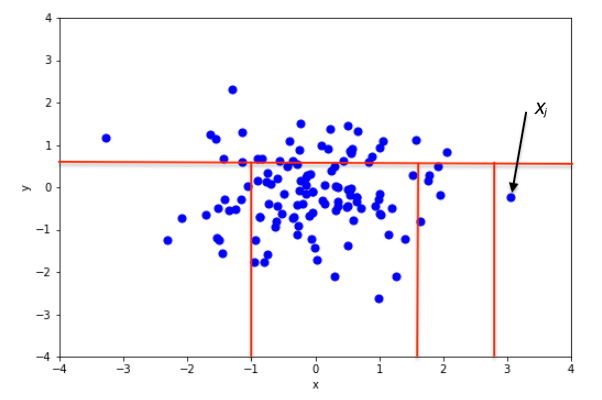
\includegraphics[width=\linewidth]{body/02_methodology/img/figure4.png}
  \caption{An example of isolating an anomalous point in a 2D Gaussian distribution after 4 phrases.}
\end{figure}

In the same way, Isolation Forest uses random questions to separate rare or unusual data points (like the rare fruits) from the common ones. By figuring out which data points need fewer questions to be isolated, Isolation Forest can quickly find the rare and unusual patterns in large sets of data, making it useful for finding things like fraud in a bunch of financial transactions!
